\begin{figure}[p]
\centering
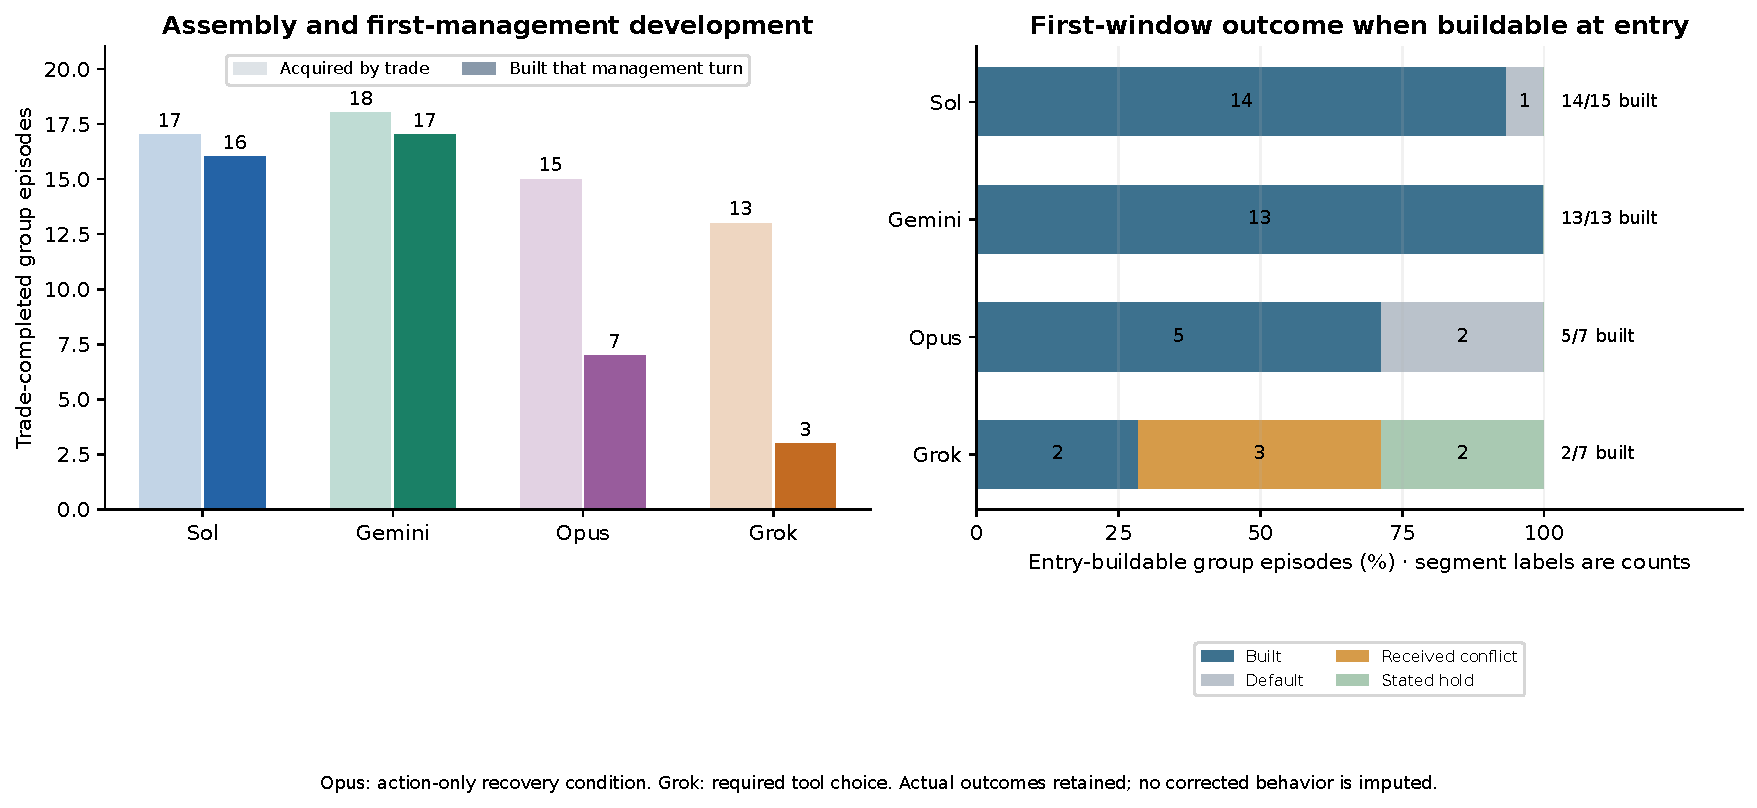
\includegraphics[width=\linewidth,height=4.4in,keepaspectratio]{f04_opportunity_and_deployment.pdf}
\caption[Trade-created opportunities and applied development]{Left: all 63 trade-completed group episodes and the 43 developed within their owner's first actual management turn. Right: 34 developed among the 42 buildable on entry, with the remaining eight visibly separated into three engine defaults, three received END/content conflicts and two consistent ENDs with stated reserve rationales. Neither panel measures willingness or overall conversion skill. Conflicts are not necessarily lost executable builds: one content plan is uneven as encoded and another requests financing. Earlier finance, jail/access and elapsed delay remain relevant. All 63 have an observed management window; 54 become buildable during it. The conditional panel cannot replace the whole path. The 113 settlements complete groups for neither/one/both sides in 60/43/10 cases; completion alone is not welfare. Sources: phase-1 accounting, phase-2 audits, Opus's residual nomination, Astra's independent original-decision check and Fable's all-63 reconstruction. Sol's final follow-up recounts those derived rows with attribution. Display next to F7 or its table. Underlying data: Table~\ref{tab:t03_trade_groups}, Table~\ref{tab:t04_bilateral_completion}, Table~\ref{tab:t09_entry_nonbuild_records}.}
\label{fig:f04_opportunity_and_deployment}
\end{figure}
